\chapter{对向量的介绍}

\section{Vector}

\begin{definition}[Vector]
    一个有序的数字列表.

    \( \left[\begin{array}{c}-1.1 \\ 0.0 \\ 3.6 \\ -7.2\end{array}\right] \) 或者 \( \quad\left(\begin{array}{c}-1.1 \\ 0.0 \\ 3.6 \\ -7.2\end{array}\right) \) 或者 \( \quad(-1.1,0,3.6,-7.2) \)
\end{definition}

表中的数字是\textit{元素}(\textit{项、系数、分量}). 元素的数量是向量的\textit{大小}(\textit{维数, 长度}). 大小为$n$的向量称为\textit{$n$维向量}. 
向量中的数字通常被称作\textit{标量}. 

用符号来表示向量, 比如$\alpha$ , $b$, 一般用小写字母表示向量. 其它表示形式如 $\boldsymbol{g}, \vec{a}$ 等。

\begin{definition}[n维向量 \( a \) 的第 \( i \) 元素]
    $n$维向量 \( a \) 的第\( i \) 元素表示为 \( a_{i} \).

    有时$i$指的是向量列表中的第$i$个向量.
\end{definition}

\begin{definition}[$a=b$]
    对于所有$i$, 如果有$a_i = b_i$, 则称两个相同大小的向量$a$和$b$是相等的, 可写成$a = b$。
\end{definition}

\begin{definition}[stacked vector]
    假设$b$、$c$、$d$是大小为$m$、$n$、$p$的向量
    
    $$ a=\left[\begin{array}{l}b \\ c \\ d\end{array}\right] $$

    $$ a=\left(b_{1}, b_{2}, \ldots, b_{m}, c_{1}, c_{2}, \ldots, c_{n}, d_{1}, d_{2}, \ldots, d_{p}\right) $$
\end{definition}

\begin{definition}[Subvectors]
    Colon notation can be used to define subvectors (slices) of a vector.

    If $ a $ is a vector, then $ a_{r: s} $ is the vector of size $ s-r+1 $, with entries $ a_{r}, \ldots, a_{s} $ :
    $$
    a_{r: s}=\left(a_{r}, \ldots, a_{s}\right)
    $$

    The subscript $ r:s $ is called the \term{index range}. 
\end{definition}

Thus, in our example above, we have
    $$
    b=a_{1: m}, \quad c=a_{(m+1):(m+n)}, \quad d=a_{(m+n+1):(m+n+p)} .
    $$

\begin{remark}
    在本书中,下标从1开始。
\end{remark}

\begin{definition}[零向量]
    所有项为$0$的$n$维向量表示为$0_n$或者$0$.
\end{definition}

\begin{definition}[全一向量]
      所有项为1的$n$维向量表示为$\boldsymbol{1}_n$或者$1$.
\end{definition}

\begin{definition}[单位向量]
    当第$i$项为$1$, 其余项为$0$时表示为$e_i$
\end{definition}

\begin{example}
    $$ {e}_{1}=\left[\begin{array}{l}1 \\ 0 \\ 0\end{array}\right], \quad e_{2}=\left[\begin{array}{l}0 \\ 1 \\ 0\end{array}\right], \quad e_{3}=\left[\begin{array}{l}0 \\ 0 \\ 1\end{array}\right] $$
\end{example}

\begin{definition}[稀疏向量]
    如果一个向量的许多项都是0, 该向量为稀疏(sparse)的. 稀疏向量能在计算机上高效地存储和操作. 

$\operatorname{nnz}(x)$是指向量$x$中非零的项数(number of non-zeros), 有时用 $\ell_0$表示 . 

\end{definition}

向量 \( x=\left(x_{1}, x_{2}\right) \) 可以在二维中表示一个位置(location)或一个位移(displacement)、 图像(列向量)、 表示一句话中每个单词出现多少次、颜色等. 

\begin{example}[Monochrome (black and white) image]
    grayscale values of $ M \times N $ pixels stored as $ M N $-vector (e.g., row-wise)

    Color image: $ 3 M N $-vectors with $ \mathrm{R}, \mathrm{G}, \mathrm{B} $ values of the $ M N $ pixels

    Video: vector of size $ K M N $ represents $ K $ monochrome images of $ M \times N $ pixels
\end{example}

\begin{example}[时间序列]
    每个元素是一个样本(sample).
\end{example}

\begin{example}[自然文本进行tokenization]
    对于自然文本进行tokenization。

    将`rained'约简为`rain'称为\term{stemming}。另外会将非常常用的词,如`a', `the'和极少出现的词去掉。这些词称为停用词。
\end{example}

\begin{example}[Feature vectors]
    contain values of variables or attributes that describe members of a set.
\end{example}

\begin{remark}
    Vector elements can represent very different quantities, in different units.
\end{remark}

\begin{remark}
    It can contain categorical features (e.g., $0/1$ for male/female)
\end{remark}

\begin{remark}
    Its ordering has no particular meaning.
\end{remark}

\section{Vector Space}

\begin{definition}[向量空间$V$]
    设 \( V \) 是非空子集, \( P \) 是一数域, 向量空间$V$满足:

    \begin{enumerate}
        \item 向量加法: \( V+V \rightarrow V \), 记作 \( \forall x, y \in V \), 则 \( x+y \in V \) (加法封闭)
        \item 标量乘法: \( F \times V \rightarrow V \), 记作 \( \forall x \in V, \lambda \in P \), 则 \( \lambda x \in V \) (乘法封闭)
    \end{enumerate}


\end{definition}

\begin{theorem}
    上述两个运算满足下列八条规则 \( (\forall x, y, z \in V, \lambda, \mu \in P) \) 
\begin{enumerate}
    \item \( x+y=y+x \) (交换律) 
    \item \( x+(y+z)=(x+y)+z \) (结合律)
    \item \( V \) 存在一个零元素, 记作$0$, \( x+0=x \)
    \item 存在 \( x \) 的负元素, 记作 \( -x \), 满足 \( x+(-x)=0 \)
    \item \( \forall x \in V \), 都有 \( 1 x=x, 1 \in P \)
    \item \( \lambda(\mu x)=(\lambda \mu) x \)
    \item \( (\lambda+\mu) x=\lambda x+\mu x \)
    \item \(  \lambda(x+y)=\lambda x+\lambda y \)
\end{enumerate}
\end{theorem}

\begin{corollary}
    向量空间也称为线性空间.
\end{corollary}

\begin{corollary}
    如果 \( x, y \in \mathbb{R}^{2} \), 则 \( x+y \in \mathbb{R}^{2}, \lambda x \in \mathbb{R}^{2}(\lambda \in \mathbb{R}) \).
\end{corollary}

\begin{definition}[数域]
    数的非空集合$P$,且其中任意两个数的和、差、积、商(除数不为零)仍属于该集合, 则称数集$P$为一个数域. 
\end{definition}

\begin{example}
    有理数 $ \mathbb{Q} $
\end{example}

\begin{example}
    实数 $ \mathbb{R} $

    $ x, y \in \mathbb{R}, x=1, y=2 $
    $ x+y \in \mathbb{R}  ,x \times y \in \mathbb{R} $
\end{example}

\begin{example}
    复数 $ \mathbb{C} $
\end{example}

\section{向量运算}

\begin{definition}[向量加法]
    $n$维向量$a$和$b$可以相加, 求和形式表示为$a + b$.
\end{definition}

\begin{theorem}
    设向量 \( a, {b}, {c} \) 是向量空间 \( V \) 的元素, 即 \( a, {b}, {c} \in V_{\text {.  }} \)。向量加法满足以下性质:

    \begin{enumerate}
        \item 交换律: \( a+b=b+a \)
        \item 结合律: \( (a+b)+c=a+(b+c) \) (因此可写成 \( a+{b}+{c}) \)
        \item \( a+0=0+a=a \)
        \item \( a-a=0 \)
    \end{enumerate}
\end{theorem}

\begin{corollary}[向量位移相加]
    如果二维向量$a$和$b$都表示位移, 则它们的位移之和为$a + b$。
\end{corollary}

\begin{example}
    点$q$到点$p$的位移是$p-q$.

\begin{FigureCenter}{The translation from $q$ to $p$}
    \tikzset{every picture/.style={line width=0.75pt}} %set default line width to 0.75pt        

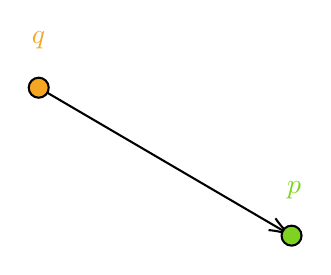
\begin{tikzpicture}[x=0.75pt,y=0.75pt,yscale=-1,xscale=1]
%uncomment if require: \path (0,300); %set diagram left start at 0, and has height of 300

%Straight Lines [id:da6747700231115574] 
\draw    (104.82,116.82) -- (224.91,187.09) ;
\draw [shift={(226.64,188.1)}, rotate = 210.34] [color={rgb, 255:red, 0; green, 0; blue, 0 }  ][line width=0.75]    (10.93,-3.29) .. controls (6.95,-1.4) and (3.31,-0.3) .. (0,0) .. controls (3.31,0.3) and (6.95,1.4) .. (10.93,3.29)   ;
%Shape: Circle [id:dp2346779756728088] 
\draw  [fill={rgb, 255:red, 126; green, 211; blue, 33 }  ,fill opacity=1 ] (221.82,188.1) .. controls (221.82,185.44) and (223.97,183.29) .. (226.64,183.29) .. controls (229.3,183.29) and (231.45,185.44) .. (231.45,188.1) .. controls (231.45,190.76) and (229.3,192.92) .. (226.64,192.92) .. controls (223.97,192.92) and (221.82,190.76) .. (221.82,188.1) -- cycle ;
%Shape: Circle [id:dp32683820972368327] 
\draw  [fill={rgb, 255:red, 245; green, 166; blue, 35 }  ,fill opacity=1 ] (100,116.82) .. controls (100,114.16) and (102.16,112) .. (104.82,112) .. controls (107.48,112) and (109.64,114.16) .. (109.64,116.82) .. controls (109.64,119.48) and (107.48,121.64) .. (104.82,121.64) .. controls (102.16,121.64) and (100,119.48) .. (100,116.82) -- cycle ;

% Text Node
\draw (100,88.4) node [anchor=north west][inner sep=0.75pt]  [color={rgb, 255:red, 245; green, 166; blue, 35 }  ,opacity=1 ]  {$q$};
% Text Node
\draw (223,160.4) node [anchor=north west][inner sep=0.75pt]  [color={rgb, 255:red, 126; green, 211; blue, 33 }  ,opacity=1 ]  {$p$};


\end{tikzpicture}
\end{FigureCenter} 


\end{example}

\begin{definition}[标量与向量的乘法]
    $$ \beta a=\left[\begin{array}{c}\beta a_{1} \\ \vdots \\ \beta a_{n}\end{array}\right] $$
\end{definition}

\begin{theorem}
    标量 \( \beta, \gamma \) 与向量 \( a 、 b \)进行乘法, 有如下性质:
    \begin{enumerate}
        \item 结合律: \( (\beta \gamma) a=\beta(\gamma a) \)
        \item 左分配律: \( (\beta+\gamma) a=\beta a+\gamma a \)
        \item 右分配律: \( \beta(a+b)=\beta a+\beta b \)
    \end{enumerate}
\end{theorem}

\begin{definition}[线性组合]
    对于向量 \( a_{1}, \ldots, a_{m} \) 和标量 \( \beta_{1}, \ldots, \beta_{m} \),
    $$ \beta_{1} a_{1}+\cdots+\beta_{m} a_{m} $$
    是向量的线性组合. \( \beta_{1}, \ldots, \beta_{m} \) 是该向量的\textit{系数}. 
\end{definition}



    \begin{theorem}
        对于任何向量 \( b \in \mathbb{R}^{n} \), 满足
    $$ b=b_{1} e_{1}+\cdots+b_{n} e_{n}, b=\left[\begin{array}{c}b_{1} \\ b_{2} \\ \vdots \\ b_{n}\end{array}\right] $$
    \end{theorem}
    
    $ \beta_{1}=\cdots=\beta_{m}=1 $时,线性组合是$a_1, \cdots, a_m$的和。

    $ \beta_{1}=\cdots=\beta_{m} = \frac{1}{m} $时,线性组合是$a_1, \cdots, a_m$的平均。

    When the coefficients sum to one, i.e., $ \beta_{1}+\cdots+\beta_{m}=1 $, the linear combination is called an \term{affine combination}. When the coefficients in an affine combination are nonnegative, it is called a \term{convex combination}, a \term{mixture}, or a \term{weighted average}. The coefficients in an affine or convex combination are sometimes given as percentages, which add up to $ 100 \% $.

\section{内积}

\begin{definition}[内积]
    在数域 \( \mathbb{R} \) 上的向量空间 \( V \), 定义函数 \( \langle\cdot,\cdot\rangle:V \times V \rightarrow \mathbb{R} \), 满足:

    \begin{enumerate}
        \item $ \langle{a}, {a}\rangle \geq 0, \forall {a} \in V $, 当且仅当 $a=0$ 时 $ \langle a, a\rangle=0 $.
        \item \( \langle\alpha {a}+\beta {b}, c\rangle=\alpha\langle{a}, c\rangle+\beta\langle{b}, c\rangle, \forall \alpha, \beta \in \mathbb{R} \), 且 \( {a}, {b}, c \in V \).
        \item \( \langle{a}, {b}\rangle=\langle{b}, {a}\rangle, \forall {a}, {b} \in V \).
    \end{enumerate}

    则称函数 \( \langle\cdot,\cdot\rangle:V \times V \rightarrow \mathbb{R} \)是内积. 
\end{definition}

\begin{example}[the inner product of two $ n $-vectors $ a, b $]
    在向量空间 \( \mathbb{R}^{n} \) 上,  计算两个向量对应项相乘之后求和函数
    $$ \langle a, b\rangle=a_{1} b_{1}+a_{2} b_{2}+\cdots+a_{n} b_{n}=a^{T}{b} $$

where \( a=\left[\begin{array}{c}a_{1} \\ a_{2} \\ \vdots \\ a_{n}\end{array}\right], b=\left[\begin{array}{c}b_{1} \\ b_{2} \\ \vdots \\ b_{n}\end{array}\right] \in \mathbb{R}^{n} \).
\end{example}

\begin{proof}
对于性质1
    $$\langle a, a\rangle=a^T a=a_{1} a_{1}+a_{2} a_{2}+\cdots+a_{n} a_{n}=\sum_{i=1}^{n} a_{i}^{2} \geq 0,$$

    $\langle a, a\rangle=0 则 a=0$.

    对于性质2
    $$\begin{aligned} \langle\alpha a+\beta {b}, {c}\rangle 
    & = (\alpha a+\beta {b})^T c 
    \\ &=\left(\alpha a_{1}+\beta b_{1}\right) c_{1}+\left(\alpha a_{2}+\beta b_{2}\right) c_{2}+\cdots+\left(\alpha a_{n}+\beta b_{n}\right) c_{n} 
    \\ &=\alpha \sum_{i=1}^{n} a_{i} c_{i}+\beta \sum_{i=1}^{n} b_{i} c_{i}
    \\ &=\alpha\langle a, c\rangle+\beta\langle b, c\rangle\end{aligned} $$

    对于性质3
    $$ \langle a, b\rangle=a^{{T}} b=b^{{T}} a=\langle b, a\rangle $$
\end{proof}

\begin{theorem}
    内积的性质:交换律、结合律、分配律. 

交换律(commutative): \( a^{T} b=b^{T} a \)

结合律(associative with scalar multiplication): \( (\gamma a)^{T} b=\gamma\left(a^{T} b\right) \)

分配律(distributive with vector addition): \( (a+b)^{T} c=a^{T} c+b^{T} c \)
\end{theorem}


\subsection{常用的内积等式}
\begin{corollary}[选出第$i$项]
    $$ e_{i}^{T} a=a_{i} $$
\end{corollary}

\begin{corollary}[向量每一项之和]
    $$ \mathbf{1}^{T} a=a_{1}+\cdots+a_{n} $$
\end{corollary}

\begin{corollary}[向量每一项的平方和]
    $$ a^{T} a=a_{1}^{2}+\cdots+a_{n}^{2} $$
\end{corollary}

\begin{corollary}[向量元素的平均值]
    $$ (\frac{\mathbf{1}}{n})^{T} a= \frac{a_{1}+\cdots+a_{n}}{n}  $$
\end{corollary}

\begin{corollary}[Selective sum]
    Let $ b $ be a vector all of whose entries are either 0 or 1 . Then $$ b^{T} a $$ is the sum of the elements in $ a $ for which $ b_{i}=1 $.
\end{corollary}

\begin{corollary}[Differencing]
    $$ \left(e_{i}-e_{j}\right)^{T} a=a_{i}-a_{j} $$
\end{corollary}

\begin{definition}[The sum of block vectors]
    If the vectors $ a $ and $ b $ are block vectors, and the corresponding blocks have the same sizes (in which case we say they \textit{conform}), then 

    $$ a^{T} b=\left[\begin{array}{c}a_{1} \\ \vdots \\ a_{k}\end{array}\right]^{T}\left[\begin{array}{c}b_{1} \\ \vdots \\ b_{k}\end{array}\right]=a_{1}^{T} b_{1}+\cdots+a_{k}^{T} b_{k} $$
\end{definition}


\section{Examples for Inner Product}

内积用途很广.

\begin{example}[计算同时出现的项目数]
   $$
a=(0,1,1,1,1,1,1), \quad b=(1,0,1,0,1,0,0)
$$
Here we have $ a^{T} b=2 $, which is the number of objects in both $ A $ and $ B $ (i.e., objects 3 and 5). 
\end{example}

\begin{example}[Weights, features, and score]
    When the vector $f$ represents a set of \textit{features} of
    an object, and $w$ is a vector of the same size (often called a \textit{weight vector}), the
    inner product $w^T f$ is the sum of the feature values, scaled (or weighted) by
    the weights, and is sometimes called a \textit{score}.

    Inner product $ w^{T} f=w_{1} f_{1}+w_{2} f_{2}+\cdots+w_{n} f_{n} $ is total score. 

\end{example}

\begin{example}[多项式]
    Suppose the $ n $-vector $ c $ represents the coefficients of a polynomial $ p $ of degree $ n-1 $ or less:

    $$ p(x)=c_{1}+c_{2} x+\cdots+c_{n-1} x^{n-2}+c_{n} x^{n-1} $$

    Let $t$ be a number, $ z=\left(1, t, t^{2}, \ldots, t^{n-1}\right) $  be the $n$-vector of powers
    of $t$. Then

    $$ c^{T} z=p(t) $$
\end{example}


\section{Cauchy-Schwartz Inequality}
\begin{theorem}[Cauchy-Schwartz Inequality]
    \label{thm:cauchy-schwartz=inequality}
    设 \( \langle \cdot,\cdot \rangle \) 是向量空间 \( V \) 上的内积, \( \forall x, y \in V \), 则有

    $$
|\langle x, y\rangle|^{2} \leq\langle x, x\rangle\langle y, y\rangle
$$

    当$x=-\lambda y$时,有$|\langle x, y\rangle|^{2}=\langle x, x\rangle\langle y, y\rangle$。
\end{theorem}

\begin{proof}
    令 $\lambda \in \mathbb{R}$, 则有 
    $$0 \leq\langle x+\lambda y, x+\lambda y\rangle=\langle x, x\rangle+\lambda\langle y, x\rangle+\lambda\langle x, y\rangle+\lambda^{2}\langle y, y\rangle=\langle x, x\rangle+2 \lambda\langle y, x\rangle+\lambda^{2}\langle y, y\rangle$$

则 
$$\lambda^{2}\langle y, y\rangle+2 \lambda\langle y, x\rangle+\langle x, x\rangle \geq 0, \forall \lambda \in \mathbb{R}$$

所以
$$
\begin{aligned}
&\nabla=(2\langle y, x\rangle)^{2}-4\langle y, y\rangle\langle x, x\rangle \leq 0 \\
&|\langle x, y\rangle|^{2} \leq\langle x, x\rangle\langle y, y\rangle
\end{aligned}
$$

当 $|\langle x, y\rangle|^{2}=\langle x, x\rangle\langle y, y\rangle$ 时, 有 $$\langle x, x\rangle^{2}+2 \lambda\langle y, x\rangle+\lambda^{2}\langle y, y\rangle=0$$

也即 $$\langle x+\lambda y, x+\lambda y\rangle=0$$

因此 $x+\lambda y=0$, 即 $x=-\lambda y$。
\end{proof}

\begin{theorem}[Cauchy-Schwarz 不等式的矩阵元素形式]

    $$\left(\sum_{i=1}^{n} u_{i} v_{i}\right)^{2} \leq\left(\sum_{i=1}^{n} u_{i}^{2}\right)\left(\sum_{i=1}^{n} v_{i}^{2}\right)$$
\end{theorem}

\begin{proof}
    The Cauchy-Schwarz inequality can be proved using only ideas from elementary algebra in this case. Consider the following quadratic polynomial in $x$
$$
0 \leq\left(u_{1} x+v_{1}\right)^{2}+\cdots+\left(u_{n} x+v_{n}\right)^{2}=\left(\sum_{i} u_{i}^{2}\right) x^{2}+2\left(\sum_{i} u_{i} v_{i}\right) x+\sum_{i} v_{i}^{2}
$$
Since it is nonnegative, it has at most one real root for $x$. Hence its discriminant is less than or equal to zero. That is,
$$
\Delta = \left(\sum_{i} u_{i} v_{i}\right)^{2}-\left(\sum_{i} u_{i}^{2}\right)\left(\sum_{i} v_{i}^{2}\right) \leq 0
$$
which yields the Cauchy-Schwarz inequality.
\end{proof}

\begin{corollary}[Cauchy-Schwarz不等式的等价形式]
    由Cauchy-Schwarz不等式
    $$
    |\langle x, y\rangle|^{2} \leq\langle x, x\rangle\langle y, y\rangle
    $$

    可以推得
    $$\begin{aligned}
        |\langle a,b \rangle| &\le \| a \|_2 \| b \|_2\\
        \langle a,b \rangle &\ge -\| a \|_2 \| b \|_2
    \end{aligned} $$
\end{corollary}


\section{浮点运算}

计算机以浮点格式存储(实)数值. 存储$n$维的向量需要$8n$字节进行存储。

基本的算术运算(加法, 乘法等)被称为浮点运算(flop). 

\begin{definition}[Floating point operation (flop)]
    the unit of complexity when comparing vector and matrix algorithms.

    1 flop $ = $ one basic arithmetic operation $ (+,-, *, /, \sqrt{,} \ldots) $ in $ \mathbf{R} $ or $ \mathbf{C} $.
\end{definition}

\begin{remark}
    This is a very simplified model of complexity of algorithms.

    \begin{itemize}
        \item we don't distinguish between the different types of arithmetic operations
        \item we don't distinguish between real and complex arithmetic
        \item we ignore integer operations (indexing, loop counters, ...)
        \item we ignore cost of memory access
    \end{itemize}
\end{remark}

算法或操作的时间复杂度:作为输入维数的函数所需要的浮点运算总数。算法复杂度通常以非常粗略地近似估算。(程序)执行时间的粗略估计:计算机速度/flops,目前的计算机大约是$1$Gflops/秒($10^9$flops/秒)。

\begin{definition}[Operation count (flop count)]
    Total number of operations in an algorithm. In linear algebra, it is typically a polynomial of the dimensions in the problem

\end{definition}
\begin{theorem}[通过浮点运算次数大致预测程序的运行时间]
    a crude predictor of run time of the algorithm.

    $$\text{run time}  \approx \frac{\text { number of operations (flops) }}{\text { computer speed (flops per second) }} $$
\end{theorem}

\begin{definition}[Dominant term]
    The highest-order term in the flop count.

\end{definition}

\begin{example}
    $$
\frac{1}{3} n^{3}+100 n^{2}+10 n+5 \approx \frac{1}{3} n^{3}
$$
\end{example}

\begin{definition}[Order]
    The power in the dominant term.
\end{definition}

\begin{example}
    $$
\frac{1}{3} n^{3}+10 n^{2}+100=\text { order } n^{3}
$$
\end{example}


\begin{corollary}
    假设有$n$维向量$x$和$y$

    \begin{itemize}
        \item $x+y$需要$n$次加法, 所以时间复杂度为 ($n$)flops. 
        \item $x^T y$ 需要$n$次乘法和$n - 1$次加法, 所以时间复杂度为$(2n - 1)$flops. 
        \item 对于$x^T y$, 通常将其时间复杂度简化为$2n$, 甚至为$n$. 
        \item 当$x$或$y$是稀疏的时候, 算法的实际运算时间会比理论时间更少. 
    \end{itemize}
\end{corollary}


\section{Complex numbers and Vectors}

\begin{definition}[Complex Numbers]
    $ x=\alpha+\mathrm{j} \beta $ with $ \alpha, \beta $ real scalars

    $ \mathrm{j}=\sqrt{-1} $ (more common notation is $ i $ or $ j $ ), $ \alpha $ is the \term{real} part of $ x $, denoted $ \operatorname{Re} x $, $ \beta $ is the \term{imaginary} part, denoted $ \operatorname{Im} x $
\end{definition}

\begin{definition}[Set of complex numbers]
    set of complex numbers is denoted $ \mathbf{C} $
\end{definition}

\begin{definition}[Modulus]
    modulus (absolute value, magnitude): $$ |x|=\sqrt{(\operatorname{Re} x)^{2}+(\operatorname{Im} x)^{2}} $$
\end{definition}

\begin{definition}[Conjugate]
    $$ \bar{x}=\operatorname{Re} x-\mathrm{j} \operatorname{Im} x $$
\end{definition}

\begin{theorem}
    $$ \operatorname{Re} x=\frac{x+\bar{x}}{2} $$
\end{theorem}

\begin{theorem}
    $$ \operatorname{Im} x=\frac{x-\bar{x}}{2 \mathrm{j}} $$
\end{theorem}

\begin{theorem}
    $$ |x|^{2}=\bar{x} x $$
\end{theorem}

\subsection{Polar representation}

\begin{theorem}
    nonzero complex number $ x=\operatorname{Re} x+\mathrm{j} \operatorname{Im} x $ can be written as
$$
x=|x|(\cos \theta+\mathrm{j} \sin \theta)=|x| e^{\mathrm{j} \theta}
$$

$ \theta \in[0,2 \pi) $ is the \term{argument} (\term{phase angle}) of $ x $ (notation: $ \arg x $ ). $ e^{\mathrm{j} \theta} $ is complex exponential.
\end{theorem}

\begin{theorem}[Euler's formula]
    $ e^{\mathrm{j} \theta}=\cos \theta+\mathrm{j} \sin \theta $
\end{theorem}

\begin{FigureCenter}{Complex Numbers}
    

\tikzset{every picture/.style={line width=0.75pt}} %set default line width to 0.75pt        

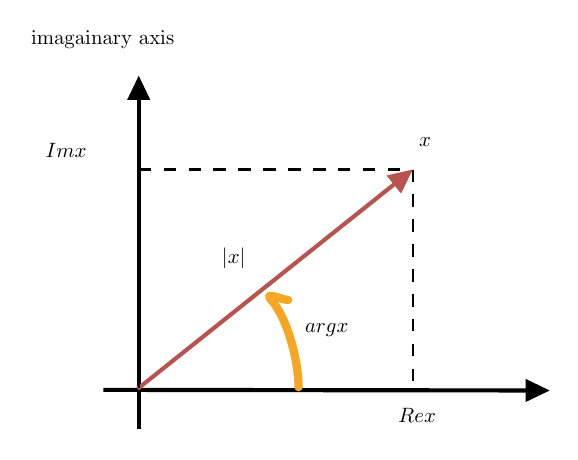
\begin{tikzpicture}[x=0.75pt,y=0.75pt,yscale=-1,xscale=1]
%uncomment if require: \path (0,300); %set diagram left start at 0, and has height of 300

%Straight Lines [id:da4158839935279788] 
\draw [line width=1.5]    (267,233) -- (478,233.3) ;
\draw [shift={(482,233.3)}, rotate = 180.08] [fill={rgb, 255:red, 0; green, 0; blue, 0 }  ][line width=0.08]  [draw opacity=0] (11.61,-5.58) -- (0,0) -- (11.61,5.58) -- cycle    ;
%Straight Lines [id:da5390398615537384] 
\draw [line width=1.5]    (284,252) -- (284,85.68) ;
\draw [shift={(284,81.68)}, rotate = 90] [fill={rgb, 255:red, 0; green, 0; blue, 0 }  ][line width=0.08]  [draw opacity=0] (11.61,-5.58) -- (0,0) -- (11.61,5.58) -- cycle    ;
%Straight Lines [id:da928526944402611] 
\draw [color={rgb, 255:red, 184; green, 84; blue, 80 }  ,draw opacity=1 ][fill={rgb, 255:red, 184; green, 84; blue, 80 }  ,fill opacity=1 ][line width=1.5]    (283.5,232.5) -- (412.87,129.33) ;
\draw [shift={(416,126.84)}, rotate = 141.43] [fill={rgb, 255:red, 184; green, 84; blue, 80 }  ,fill opacity=1 ][line width=0.08]  [draw opacity=0] (11.61,-5.58) -- (0,0) -- (11.61,5.58) -- cycle    ;
%Shape: Rectangle [id:dp5932303428508245] 
\draw  [dash pattern={on 4.5pt off 4.5pt}] (284,126.84) -- (416,126.84) -- (416,233.5) -- (284,233.5) -- cycle ;
%Shape: Free Drawing [id:dp3532268261143874] 
\draw  [color={rgb, 255:red, 245; green, 166; blue, 35 }  ,draw opacity=1 ][line width=3] [line join = round][line cap = round] (361,231.7) .. controls (361,218.56) and (355.2,196.89) .. (347,188.7) ;
%Shape: Free Drawing [id:dp6391532692612814] 
\draw  [color={rgb, 255:red, 245; green, 166; blue, 35 }  ,draw opacity=1 ][line width=3] [line join = round][line cap = round] (347,187.7) .. controls (350.61,187.7) and (353.29,189.7) .. (356,189.7) ;


% Text Node
\draw (238,113) node [anchor=north west][inner sep=0.75pt]  [xscale=0.75,yscale=0.75] [align=left] {$\displaystyle \operatorname{Im} x$};
% Text Node
\draw (408,241) node [anchor=north west][inner sep=0.75pt]  [xscale=0.75,yscale=0.75] [align=left] {$\displaystyle \operatorname{Re} x$};
% Text Node
\draw (231,59) node [anchor=north west][inner sep=0.75pt]  [xscale=0.75,yscale=0.75] [align=left] {imagainary axis};
% Text Node
\draw (418,110.4) node [anchor=north west][inner sep=0.75pt]  [xscale=0.75,yscale=0.75]  {$x$};
% Text Node
\draw (323,163.4) node [anchor=north west][inner sep=0.75pt]  [xscale=0.75,yscale=0.75]  {$| x| $};
% Text Node
\draw (363,200) node [anchor=north west][inner sep=0.75pt]  [xscale=0.75,yscale=0.75] [align=left] {$\displaystyle \operatorname{arg} x$};


\end{tikzpicture}
\end{FigureCenter}

\subsection{Complex vector}

\begin{definition}[vector with complex elements]
    $ a=\alpha+\mathrm{j} \beta $ with $ \alpha, \beta $ real vectors
\end{definition}

\begin{definition}[real and imaginary part, conjugate of complex numbers]
    real and imaginary part, conjugate are defined componentwise:

$$
\begin{aligned}
\operatorname{Re} a &=\left(\operatorname{Re} a_{1}, \operatorname{Re} a_{2}, \ldots, \operatorname{Re} a_{n}\right) \\
\operatorname{Im} a &=\left(\operatorname{Im} a_{1}, \operatorname{Im} a_{2}, \ldots, \operatorname{Im} a_{n}\right) \\
\bar{a} &=\operatorname{Re} a-\mathrm{j} \operatorname{Im} a
\end{aligned}
$$
\end{definition}

\begin{definition}[ set of complex $n$-vectors]
    $$ \mathbf{C}^{n} $$
\end{definition}

\begin{definition}
    $$ a+b=\left[\begin{array}{c}a_{1}+b_{1} \\ a_{2}+b_{2} \\ \vdots \\ a_{n}+b_{n}\end{array}\right], \quad \gamma a=\left[\begin{array}{c}\gamma a_{1} \\ \gamma a_{2} \\ \vdots \\ \gamma a_{n}\end{array}\right], \quad a \circ b=\left[\begin{array}{c}a_{1} b_{1} \\ a_{2} b_{2} \\ \vdots \\ a_{n} b_{n}\end{array}\right] $$
\end{definition}

\begin{definition}[Complex inner product]
    the inner product of complex $ n $-vectors $ a, b $ is defined as
$$
b^{H} a=\bar{b}_{1} a_{1}+\bar{b}_{2} a_{2}+\cdots+\bar{b}_{n} a_{n}
$$
\end{definition}

other notation: $ \langle a, b\rangle,(a \mid b), \ldots $.

for real vectors, reduces to real inner product $ b^{T} a $.

for complex $ n $-vectors $ a, b, c $ and complex scalars $ \gamma $

$a^H a$有如下性质:
\begin{theorem}
    $ a^{H} a \geq 0 $ : follows from
$$
\begin{aligned}
a^{H} a &=\bar{a}_{1} a_{1}+\bar{a}_{2} a_{2}+\cdots+\bar{a}_{n} a_{n} \\
&=\left|a_{1}\right|^{2}+\left|a_{2}\right|^{2}+\cdots+\left|a_{n}\right|^{2}
\end{aligned}
$$

\end{theorem}

\begin{theorem}
    $$ a^{H} a=0 \text{ only if } a=0 $$
\end{theorem}

\begin{theorem}
    $$ b^{H} a=\overline{a^{H} b} $$
\end{theorem}

\begin{theorem}
    $$ (\gamma b)^{H} a=\bar{\gamma}\left(b^{H} a\right) $$
\end{theorem}

\begin{theorem}
    $$ (b+c)^{H} a=b^{H} a+c^{H} a $$
\end{theorem}

\begin{theorem}
    $$ b^{H}(a+c)=b^{H} a+b^{H} c $$
\end{theorem}

\begin{theorem}
    $$ b^{H}(\gamma a)=\gamma\left(b^{H} a\right) $$
\end{theorem}